\documentclass[12pt]{article}
\usepackage{tikz}
\usetikzlibrary{shapes,snakes}
\usetikzlibrary{arrows,automata}
\usepackage{algorithm}
\usepackage{algorithmic}%\usepackage[pagebackref=true,colorlinks,linkcolor=blue,citecolor=magenta]{hyperref}
\usepackage{graphicx} 
\usepackage{fancybox}
\usepackage{setspace}  
\usepackage[colorlinks,linkcolor=blue,citecolor=magenta]{hyperref}
\usepackage{enumerate} 
%\usepackage{auto-pst-pdf} 
\usepackage{amsthm,amssymb,amsmath}
\usepackage{indentfirst}
\usepackage{listings}
\usepackage{alltt}
\usepackage{clrscode}
\renewcommand{\algorithmiccomment}[1]{// #1}
\newtheorem{theorem}{Theorem}
\begin{document}

\title{Initial Value Computation}
\author{}
\date{\today}
\maketitle
\newcommand{\dom}{\textsf{dom}}

\section{Definitions}
In this draft we want to explain the notion of domains. The domain of a variable is the set of values that it can take. The domain of all the variables in a query expression can easily be computed recursively if some rules are respected. We will use through out the entire paper the notation of $\text{\dom{}}_{\vec x}(q)$ for the domain of a set of variables, where $q$ is the given query and $\vec x$ is a vector representing the variables(not necessarily present in the expression $q$). Taking into account the expressions from the AGCA (Aggregate Calculus\cite{1}) the definition of an expression will be: 
$$q\text{ ::- }q\cdot q | q + q|v \gets q |v_{1}\theta v_{2}|R(\vec{y})|\text{constant}|\text{variable}$$

We start with the definition of $\dom{}_{\vec x}(R(\vec y))$:
$$\dom{}_{\vec x}(R(\vec y))=\bigg\{\vec c\,\Big|\,(\prod_{i:x_{i}\in \vec y}^{}(x_{i}\gets c_{i})\cdot R(\vec y))\not= 0\bigg\} $$where $\vec x=<x_1,x_2,x_3,\cdots,x_i,\cdots>$, $\vec c=<c_1,c_2,c_3,\cdots,c_i,\cdots>$.  $\vec{x}$ defines the schema of $\vec{c}$, specifically, $\vec{x}$ is a vector of names of each element of the tuple $\vec{c}$. It is not necessary that $\vec{x}$  has the same schema as the given expression. Thus, we can evaluate $\text{\dom}_{\vec{x}}$ for a broader range of $\vec{x}$ and it is not restricted by the schema of the input query expression. In such cases the \dom{} is infinite as the not presenting variables in the query can take any value.\\
\par
For the comparison operator ($v_{1}\theta v_{2}$), where $v_1$ and $v_2$ are variables, we can compute the domain as follows:
\begin{equation*}
\text{\dom{}}_{\vec{x}}(v_{1}\theta v_{2})=\bigg\{\vec{c}\,\Big|\,\Big(\big(\prod_{i}(x_{i}\gets c_{i})\big)(v_{1}\theta v_{2})\Big)\not= 0\bigg\}
\end{equation*}
The domain of a comparison may be infinite. For the join operator we can write:
\begin{equation*}
\text{\dom{}}_{\vec{x}}(q_{1}\cdot q_{2})=\{\vec{c}\,|\vec{c}\in\text{\dom{}}_{\vec{x}}(q_{1})\land\vec{c}\in\text{\dom{}}_{\vec{x}}(q_{2})\}
\end{equation*}
while for the union operator the domain definition is very similar:
\begin{equation*}
\text{\dom{}}_{\vec{x}}(q_{1}+ q_{2})=\{\vec{c}\,|\vec{c}\in\text{\dom{}}_{\vec{x}}(q_{1})\lor\vec{c}\in\text{\dom{}}_{\vec{x}}(q_{2})\}
\end{equation*}
$$\dom{}_{\vec x}(constant)=\Big\{\vec c\Big\}$$
$$\dom{}_{\vec x}(variable)=\Big\{\vec c\Big\}$$

Finally, we can give a formalism for expressing the domain of a variable that will participate in an assignment operation:
\begin{equation*}
\text{\dom{}}_{\vec{x}}(v\gets q_{1})=\bigg\{\vec{c}\,\Big|\vec{c}\in\text{\dom{}}_{\vec{x}}(q_{1})\land \bigg(\forall i:(x_{i}=v)\Rightarrow\Big(\big(q_{1}\cdot\prod_{j:x_{j}\neq v } (x_{j}=c_{j})\big)=c_{i}\Big)\bigg)\bigg\}
\end{equation*}
In fact using implication operator in the above definition allows us to extend the $\vec{x}$ to whatever vector we want, as we already said the schema of $\vec{x}$ is not necessarily the same as the schema of $q$. \\
%The \dom{} of a map is defined by all the values of both the input and output variables(which are represented as vectors). 
%\begin{equation*}
%\text{\dom}_{i}=  \big\{x\in map_{i}[\vec{x}][\vec{y}]| (x\in \vec{x})\lor(x\in \vec{y})\big\}
%\end{equation*}
%We need to compute the dependences between the domains of maps.The domains of input variables will always depend on the domains of output variables from maps that are on the left side of the map with input variables. Without loose of generality  we always need to work with two maps when we want to compute their \dom s. For this we define function $F$ recursively as follow:
%\begin{equation*}
%F=\text{\dom}_{i}|F\cap F|F\cup F
%\end{equation*}
%Function $F$ takes two sets(two \dom s) and returns their unions or intersections. We can apply this function recursively to compute any set of unions or intersections between the \dom s. Also we can achieve this by giving a set of sets to $F$ to compute the desirable set.
%So we can compute the dependencies between the \dom s like this:
%\begin{equation*}
%\text{\dom}_{i}(x\in m_{i}[\vec{x}][\vec{y}])\gets F(\text{\dom}_{i}(x'\gets m_{j}[\vec{x'}][\vec{y'}]))
%\end{equation*}
%Where $j$ is all the maps which occurs on the left hand of phrase for computing $m_{i}$ as we have in \ref{fig1} since the information can only be passed from left to right.\\ 
%\par
%We call the arity of a schema as the number of its input variables. 
\par
Having the definitions for the domains, we will try to give some insight regarding to the notion of arity. We will start with an example relation: $$q=R(a,b)\cdot S(b,c)$$ the schema for q will have three variables $(a,b,c)$. The arity of a tuple is the number of its occurrences in the relation, in other words the order of multiplicity of that tuple. The arity of a tuple will increase or decrease if insertions or respectively deletions will be made to a relation. For example:
\begin{table}[ht]
\centering
\begin{tabular}{c c c c}
	R & a & b & arity\\ [0.2ex]
	%heading
	\hline
	  & $<$1 & 2$>$ & 1 \\
	  & $<$1 & 3$>$ & 2 \\
	  & $<$3 & 4$>$ & 1 \\
\end{tabular}
\caption{Relation $R$}
\end{table}
\begin{table}[ht]
\centering
\begin{tabular}{c c c c}
	S & b & c & arity\\ [0.2ex]
	%heading
	\hline
	  & $<$1 & 1$>$ & 1 \\
	  & $<$2 & 2$>$ & 2 \\
	  & $<$3 & 5$>$ & 2 \\
\end{tabular}
\caption{Relation $S$}
\end{table}
\begin{table}[ht]
\centering
\begin{tabular}{c c c c c}
	$R\cdot S$ & a & b & c & arity\\ [0.2ex]
	%heading
	\hline
	  & $<$1 & 2 & 2$>$ & 2 \\
	  & $<$1 & 3 & 5$>$ & 4 \\
	  & $<$3 & 4 & $*>$ & 0 \\
	  & $<*$ & 1 & 1$>$ & 0 \\
\end{tabular}
\caption{Relation $R\cdot S$}
\end{table}

We need to maintain the maps for certain values as long as the arity of a tuple is greater then 0. If the arity  of the tuple drops to 0 then the tuple will not be taken into consideration and therefore it can be eliminated from the domains of the maps.

We need to store the arities inside each map and also way to compute the arity of an AGCA expression. Since we substitute the subexpressions with maps, we can easily consider the relations as the maps without input variables. Also a map with input variables can be seen as a relation with a group-by clause. Input variable of a map bind some variables. Thus if we compute the map values by all different combinations of these variables, we will look up into these values and return the appropriate value according to the input variables.  
\section{Computing the arities of the AGCA expressions}
We define the function \emph{arity} which will be used to compute the arity of a tuple in a certain relation. The function will be defined on the relation and the tuple for which the multiplicity order is desired to be computed. $$arity(\text{Relation } q,\text{Tuple } t)=\text{multiplicity order of tuple }t\text{ in the relation } q$$ $$arity(q,t)=\pi_{t}(q)$$ where $\pi_{t}(q)$ means the projection of relation $q$ for the tuple $t$. This function can be used for the computation of the arity of the expressions from the AGCA: $q\text{ ::- }q\cdot q\text{ }|\text{ }q+q\text{ }|\text{ }q \theta t\text{ }|\text{ }t\gets q\text{ }|\text{ constant}\text{ }|\text{ variable}$. However constants and variables can be eliminated from the computation because relations are of interest.

$$arity(q_{1}\cdot q_{2},t)=\sum\limits_{\{t_{1}\}\Join \{t_{2}\}={t}}^{}arity(q_{1},t_{1})*arity(q_{2},t_{2})$$
$$arity(q_{1} + q_{2},t)=arity(q_{1},t)+arity(q_{2},t)\text{, where Schema}(q_{1})=\text{Schema}(q_{2}) $$
$$arity(v_1\text{ } \theta \text{ } v_2,t)=\begin{cases}1,& \mbox{if } v_1\theta v_2 \mbox{ is true and }v_{1}\in t \land v_{2}\in t\\
0,& \text{otherwise} \mbox{ is false} 
\end{cases}$$
$$arity(v\gets q,t)=\begin{cases}0, \mbox{ if $t\setminus\{v\}\not\in \text{\dom}_{Schema(t)}(q)$}\\ 1, \mbox{ otherwise} \end{cases}$$

%\section{Graph representation of maps}
%For computing the domains of input variables of maps we can use graph modeling. In such a way that, given the expression we can compute the domain of each expression with this modeling in $O(m\cdot p)$ where $m$ is the number of occurrences of all input variables and $p$ is the cost of evaluating the domains according to the mentioned rules. \\
%\par
%In this section firstly we talk about the the graph modeling(dependency graph), then we will give an algorithm for computing this dependency graph from the parse tree of expressions. 
%From the parse tree of an expression we can construct a directed graph $G(V,E)$. For each map $m[.][.]$ there is a vertex in $V$ and edges represent the variable. We have an edge between $m_{1}$ and $m_{2}$ with label $a$, if and only if $a$ is in the input variables of $m_{2}$ and output variables of $m_{1}$ and there is an information flow from $m_{1}$ to $m_{2}$. \\
%\par
%Obviously this graph does not have any cycle. To prove it, suppose it has a cycle with at least two vertices, call the first two vertices as $m_{1},m_{2}$. In the cycle there is an edge between $m_{1}$ and $m_{2}$. Since this is a cycle then there is a path between $m_{2}$ and $m_{1}$ also. But it is not possible because having an edge between $m_{1}$ and $m_{2}$ means that $m_{2}$ occurs after $m_{1}$ and according to information flow rule we can not have a path again between $m_{2}$ and $m_{1}$. \\
%\par
%In this graph vertices without any incoming edge are always the relations. If we evaluate the nodes with a topological traversal we can guarantee that the input variables of each maps is computed in order. The cost of domain computations is $O(m\cdot p)$, where $m$ is the number of edges in the graph and $p$ is the cost of using any of mentioned rules for computing the domain of subexpressions as we had in the aforementioned way. \\
%\par
%We can construct the graph from the given parse tree in $O(m)$ where $m$ is the number of edges. We start from the root of the parse tree and recursively compute the subgraph of the left child and right child, then we add the edges between the maps with some input variables on the right child to the appropriate vertices on the left child's graph. Since we consider each edge just one time in the algorithm, the overall order is $O(m)$. 
\section{Domain computation}

We are trying to compute the domains for each variable that appears in queries. This computation is performed on the query decomposition tree. We can traverse the tree in post order, first visiting the leaves that are represented by some relations and afterwards visiting the parent nodes and combining the relations of the children nodes. Using this technique we are trying to compute the domains, but also the vector $\vec x$ of all the variables defined in that query.\\
\par
The intuition is simple. MMM ...

The algorithm will need as inputs the root of the tree and a structure that must be previously defined and will return a structure that contains the vector of variables($x$) and the domains for each variable defined in the vector(\dom). The structure will look like:

\begin{alltt}
struct\{
x: the vector of all the variables 
dom: the domains of all the variables
\}
\end{alltt}
In \ref{alg1} we gave the function which compute this structure for the whole tree. We call it on the root and with an empty structure for $s$, computeDomain$(root,\const{nil})$. 
\begin{algorithm}[H]
\caption{computeDomains($node$,$s$)} 
\label{alg1}
\textbf{Input:} $node$ as the root of the tree to be traversed, and $s$ as the structure \\
\textbf{Output:} a structure $result$ that will contain the vector of variables $\vec x$ and the domains of each variable $\dom{}_{\vec x}(query)$
\begin{algorithmic}[1]
%\IF{$node.left\neq \const{nil}$}	%\COMMENT{A node has either 2 children or no childern}
\IF{$node.type=$``+''}
\STATE  $s_{1}\gets$ computeDomain($node$.$left, s$)
\STATE  $s_{2}\gets$ computeDomain($node.right, s$)
\STATE  $s_{3}.\vec{x}\gets s_{1}.\vec{x} \cup s_{2}.\vec{x}$ \COMMENT{this will compute the vector for all the variables, both from the right and left node}
\STATE  $s_{3}.dom\gets \text{\dom}_{s_{3}.\vec x}(node.left + node.right)$
\RETURN  $s_{3}$
\ELSIF{$node.type=$``*''}
\STATE  $s_{1} \gets \text{computeDomain}(node.left, s)$
\RETURN  computeDomain$(node.right, s_{1})$
\ELSE 
\label{line10}
\IF{$s= \const{nil}$}\label{line11}
\STATE $s_{1}.\vec{x} \gets \text{all the variables of the }node$
\STATE $s_{1}.dom \gets \dom{}_{s_{1}.\vec{x}}(node)$
\ELSE
\STATE $s_{1}.\vec{x}\gets s.\vec{x} \cup \{\text{all the variables of the $node$}\}$
\STATE $s_{1}.dom\gets \text{\dom}_{s_{1}.\vec{x}}(s.dom*\text{\dom}_{s_{1}.\vec{x}}(node))$
\ENDIF
\RETURN  $s_{1}$
\ENDIF
\end{algorithmic}
\end{algorithm}
The order of Algorithm \ref{alg1} is $O(n\cdot P)$ where $n$ is the number of nodes in the query decomposition tree and $P$ is the time needed for any rule of \dom{}'s computation, according to previous section.\\ 
\par In Algorithm \ref{alg1} we suppose that there are three types of nodes. Union nodes, join nodes and null nodes. Null nodes do not have any children. A union node or a join node always has two children so line \ref{line10} will be executed when the node is a leaf. Type field refers to the type of nodes. Also, since any node represents a query expression then we can obtain its domain with \dom{} operator as was mentioned in the previous section.\par
The ``if'' in line \ref{line11} is used to initialize structure $s$ for the first time(happens in the leftmost node of the tree).
\begin{theorem}
Algorithm \ref{alg1} compute the domains and the variables list of the given tree in $O(n\cdot P)$ correctly.  
\end{theorem}
\begin{proof}
\end{proof}
\begin{figure}[htbp]
\begin{center}
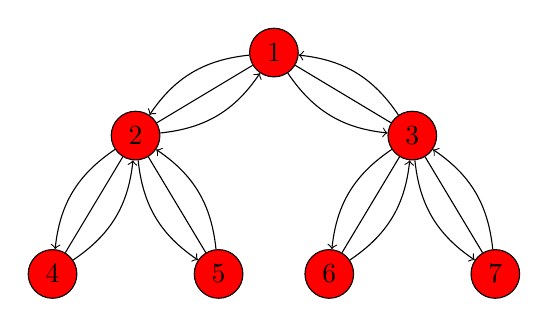
\begin{tikzpicture}%[level/.style={sibling distance=40mm,level distance=15mm}]
[level 1/.style={circle, draw,scale=1.0, fill=red,
    level distance=30pt, sibling distance=100pt},
    level 2/.style={circle, draw, scale=1.0,
    level distance=50pt, sibling distance=60pt}]
    \tikzstyle{every node}=[circle,draw,fill=red]
    \node[] (a){1}
        child { 
            node [](b){2}
            child{node(d){4}}
            child{node(e){5}} 
        }
        child { 
        		node[] (c){3}
		child{node[](f){6}}
		child{node(g){7}}
	};
	\draw[->] (a) to [bend right=25](b);
	\draw[->] (b) to [bend right=25](a);
	
	\draw[->] (a) to [bend right=25](c);
	\draw[->] (c) to [bend right=25](a);
	
	\draw[->] (b) to [bend right=25](d);
	\draw[->] (d) to [bend right=25](b);
	\draw[->] (b) to [bend right=25](e);
	\draw[->] (e) to [bend right=25](b);
	\draw[->] (c) to [bend right=25](f);
	\draw[->] (f) to [bend right=25](c);
	\draw[->] (c) to [bend right=25](g);
	\draw[->] (g) to [bend right=25](c);
	
\end{tikzpicture}
\end{center}
\caption{Tree traversal}
\label{fig1}
\end{figure}
\end{document}




